\section{Измерения}

$L = 74 \pm 0{,}5\;\text{см}$, $\lambda = 0{,}63\;\text{мкм}$, $l = 26\;\text{мм}$, $n_{o} = 2{,}29$.

\begin{tabular}{|l|l|}
\hline
$m$ & $r,\;\text{см}$\\\hline
$1{,}0$ & $2{,}8 \pm 0{,}2$\\\hline
$2{,}0$ & $3{,}9 \pm 0{,}2$\\\hline
$3{,}0$ & $4{,}8 \pm 0{,}2$\\\hline
$4{,}0$ & $5{,}5 \pm 0{,}2$\\\hline
$5{,}0$ & $6{,}1 \pm 0{,}2$\\\hline
\end{tabular}

\begin{figure}[ht!]
    \center{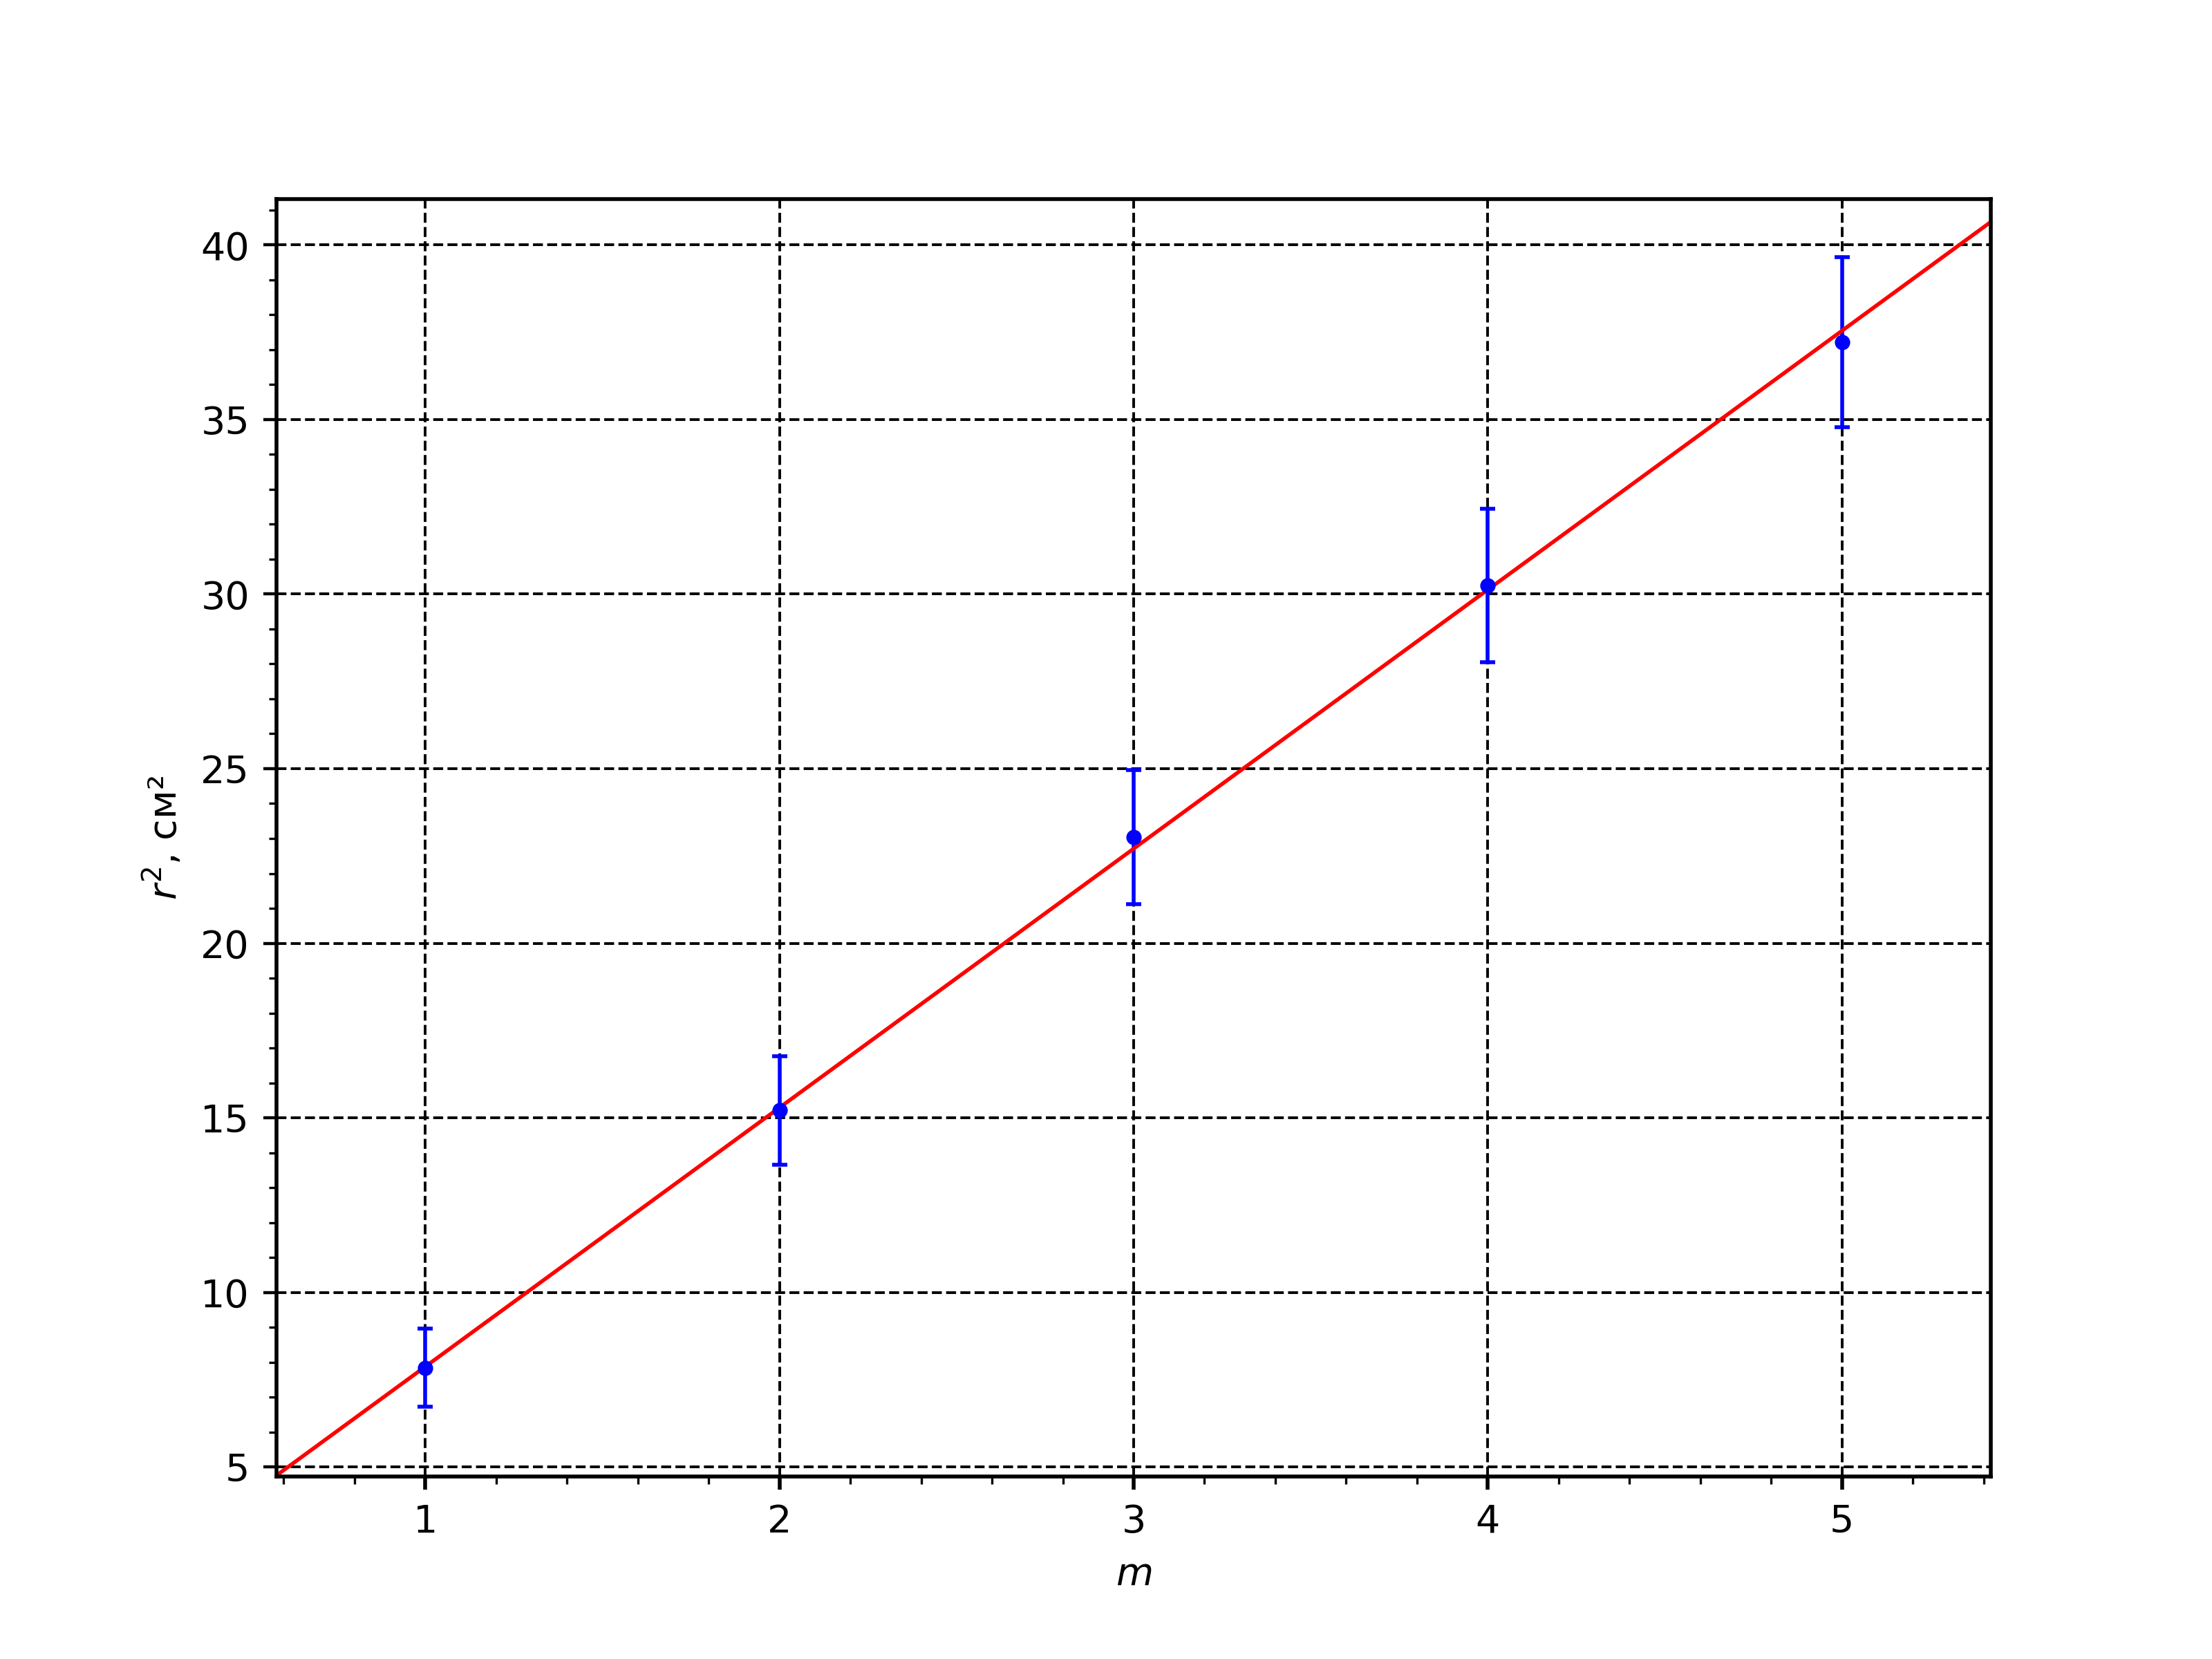
\includegraphics[width=0.8\linewidth]{../img/plot.png}}
\end{figure}

Наклон графика $k = 7{,}8 \pm 0{,}8\;\text{см}^{2}$
\[
    n_{o} - n_{e} = \frac{\left(n_{o} L\right) ^{ 2}\lambda}{lk} = 0{,}10\pm 0{,}01
\]

Методом изменения интенсивности пятна на экране найдем $U_{\lambda/2} = 480 \pm 15\;\text{В}$, $U_{\lambda} = 930\pm 15\;\text{В}$,  $U_{3\lambda/2} = 1410 \pm 15\;\text{В}$,

Методом фигур Лиссажу $U_{\lambda / 2} = 450 \pm 30\;\text{В}$

На рисунке приведены фигуры Лиссажу для случая, когда поляризации скрещены. При переходе к параллельным поляризациям они отразятся относительно горизонтальной оси.
\begin{figure}[ht!]
    \center{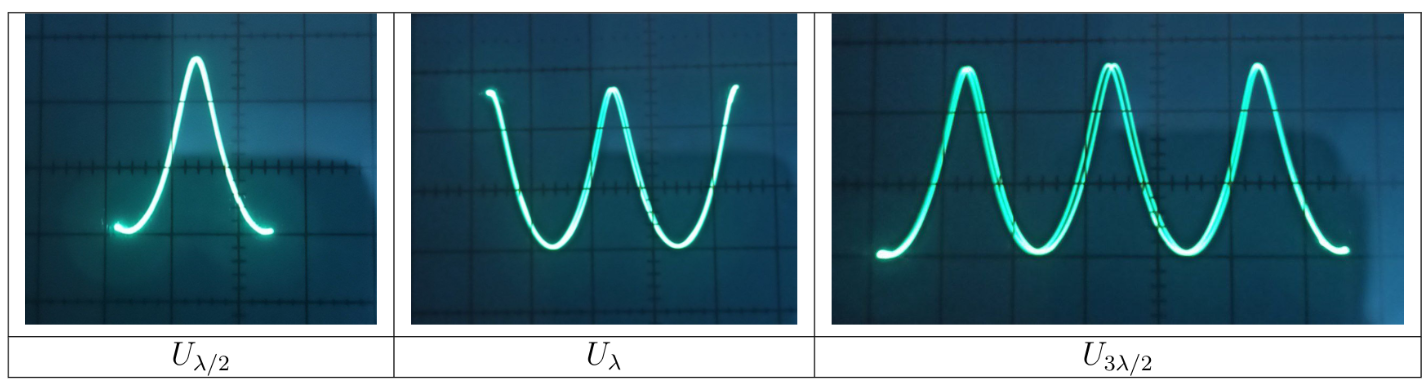
\includegraphics[width=0.8\linewidth]{../img/lis.png}}
\end{figure}

